% ---------------------------------------------------------------
% Medical Images Processing with Deep Learning (336033) - Project report
% Prose version. Max 6 pages; sections follow the course Report Guidelines.
% Every number is a measurement from outputs_fcombfix/final_eval_100k/,
% outputs_12_08_26_10000/ and outputs_11_08_26/. See RESULTS.md for the
% full experimental record.
% ---------------------------------------------------------------
\documentclass[10pt]{article}

\usepackage[margin=0.82in]{geometry}
\usepackage{amsmath}
\usepackage{graphicx}
\usepackage{booktabs}
\usepackage{xcolor}
\usepackage{tikz}
\usetikzlibrary{positioning,arrows.meta,fit,backgrounds}
\usepackage[hidelinks]{hyperref}
\setlength{\abovedisplayskip}{4pt}\setlength{\belowdisplayskip}{4pt}
\setlength{\parskip}{1pt}

\newcommand{\todo}[1]{\textcolor{red}{\textbf{[TODO: #1]}}}
\newcommand{\Dgt}{D^{\mathrm{GT}}}

\title{Disagreement-Aware Probabilistic U-Net:\\
\large Making Predictive Diversity Land Where Annotators Actually Disagree}
\author{Amit Heshes (\todo{ID}) \and Idan Smoller (\todo{ID})}
\date{\today}

\begin{document}
\maketitle
\vspace{-1.8em}

\begin{center}
\begin{minipage}{0.93\textwidth}\small
\textbf{Selected paper.} S.~A.~A. Kohl et al., \emph{A Probabilistic U-Net for
Segmentation of Ambiguous Images}, NeurIPS 2018~\cite{kohl2018}.\\
\textbf{Proposed extension.} We supervise \emph{where} human annotators disagree.
A single-convolution head predicts the inter-rater disagreement map from the
image alone, and an alignment loss drives the model's own sample diversity into
those same pixels.
\end{minipage}
\end{center}
\vspace{0.4em}

% ===============================================================
\section{Introduction}\label{sec:intro}

Semantic segmentation assigns a label to every pixel of an image, and training
normally assumes that each image has one correct mask. In medical imaging that
assumption does not hold. Several qualified experts asked to outline the same
lesion produce visibly different masks, and on the LIDC-IDRI lung-nodule dataset
they sometimes disagree about whether a lesion is present at all. A conventional
U-Net~\cite{ronneberger2015} trained on one expert's mask, or on the average of several, returns a
single confident segmentation and throws that information away precisely where it
matters most clinically.

The Probabilistic U-Net addresses this by combining a U-Net with a conditional
variational autoencoder. A prior network maps the image $x$ to a distribution
$p(z\mid x)$ over a low-dimensional latent space, and each draw of $z$ is decoded
into a different plausible segmentation. Crucially the samples are coherent whole
masks rather than independent per-pixel probabilities. This is one of the paper's
main arguments: a pixel-wise probability map cannot express which pixels vary
\emph{together}, so it cannot represent two distinct but internally consistent
readings of the same image. Training minimises the negative evidence lower bound
(ELBO), in which a posterior $q(z\mid x,Y_g)$ additionally observes one randomly
chosen expert mask $Y_g$,
\[
  L_{\text{PU-Net}}
  = \underbrace{\mathrm{E}_{z\sim q(z\mid x,Y_g)}\!\left[-\log p(Y_g\mid x,z)\right]}
      _{\text{reconstruction (cross-entropy, summed over pixels)}}
    \;+\; \beta\,\underbrace{D_{\mathrm{KL}}\!\left(q(z\mid x,Y_g)\,\|\,p(z\mid x)\right)}
      _{\text{pulls the prior towards the posterior}} ,
\]
so that at test time, sampling from the prior alone reproduces the variability
seen across annotators.

The resulting distribution of segmentations is scored with the generalized energy
distance. Writing $S,S'$ for independent model samples and $Y,Y'$ for independent
grader masks,
\[
  D^2_{\mathrm{GED}}
  = 2\,\mathrm{E}\!\left[d(S,Y)\right]
    - \underbrace{\mathrm{E}\!\left[d(S,S')\right]}_{\text{sample diversity}}
    - \mathrm{E}\!\left[d(Y,Y')\right],
  \qquad d = 1-\mathrm{IoU},
\]
where $\mathrm{IoU}(A,B)=|A\cap B|/|A\cup B|$ is the intersection over union of
two binary masks.

We chose this paper because it raised a question we found genuinely interesting:
do we always want a model to output the single answer it considers most likely?
The paper's answer is no. When the human experts themselves disagree, there is no
single correct mask to predict, and a confident deterministic output hides that.
We liked the idea of capturing the disagreement instead of averaging it away, and
wanted to take it one step further by asking not only how much the experts
disagree but \emph{where}. LIDC-IDRI makes this possible, since it provides four
independent expert masks per image, so the disagreement can be measured directly
rather than assumed.

% ===============================================================
\section{Proposed extension}\label{sec:ext}

The limitation we address is in how the paper's diversity is supervised and
scored. During training the posterior sees one randomly drawn grader per step, so
nothing in the objective ever states which \emph{parts} of the image the graders
argued about. The evaluation has the same blind spot: every term of
$D^2_{\mathrm{GED}}$ is a single number, with $\mathrm{E}[d(S,S')]$ measuring how
much the samples vary and $\mathrm{E}[d(Y,Y')]$ how much the graders vary, but
none of them asks where that variation falls. A model could therefore place the
right amount of variability in entirely the wrong region and still score well.

We expected this to be worth fixing for two reasons. First, the information is
already in the data and simply unused: four masks per image give a per-pixel
picture of the disagreement for free. Second, a model that can point at the
disputed region is more useful as a second reader than one that only reports an
overall confidence, which is the clinical motivation the paper itself opens with.
The change fits the original architecture rather than replacing it, since both of
our additions attach to the last U-Net feature map and leave the encoder,
decoder, latent space and loss of the original model intact.

Three quantities have to be kept distinct. The first, $\Dgt$, is the \emph{human}
disagreement, computed from the four masks alone. With
$P_i=\frac{1}{G}\sum_g Y_i^{(g)}$ the per-pixel mean over $G=4$ graders, $\Dgt$
is its normalised binary entropy,
\[
  \Dgt_i=-\frac{P_i\log(P_i+\epsilon)+(1-P_i)\log(1-P_i+\epsilon)}{\log 2}\in[0,1],
\]
which is $0$ wherever all four graders agree and $1$ where they split two against
two. The second, $\hat D$, is our model's \emph{prediction} of $\Dgt$. The third,
$U$, is the \emph{model} uncertainty: we draw $K$ latents from the prior, decode
each into a foreground-probability map $Q^{(k)}$, average them into
$\bar Q_i=\frac{1}{K}\sum_k Q_i^{(k)}$ and apply the same normalised binary
entropy,
\[
  U_i=-\frac{\bar Q_i\log(\bar Q_i+\epsilon)+(1-\bar Q_i)\log(1-\bar Q_i+\epsilon)}{\log 2}.
\]
Since $U$ and $\Dgt$ differ only in what is averaged, model samples in one case
and grader votes in the other, any discrepancy between them is a discrepancy of
location on a common $[0,1]$ scale. That is what makes $|U-\Dgt|$ a sensible
thing to minimise.

Our extension adds two components, both deliberately small. The
\textbf{disagreement head} is a single $1\times1$ convolution followed by a
sigmoid, applied to the last U-Net feature map and taken \emph{before} the latent
$z$ is injected, so that $\hat D$ depends on the image alone. It is trained with
$L_D=\mathrm{MSE}(\hat D,\Dgt)$. The \textbf{alignment loss}
$L_{\text{align}}=\frac{1}{HW}\sum_i|U_i-\Dgt_i|$ penalises predictive diversity
that lands anywhere other than where the graders differ, giving the full
objective $L=L_{\text{PU-Net}}+\lambda_D L_D+\lambda_A L_{\text{align}}$. In both
cases the idea is to add pixel-level information that answers the ``where''
question, while keeping the original model's view of a segmentation as a whole
coherent mask. Figure~\ref{fig:model} shows both additions in place.

% ---------------------------------------------------------------
% Figure: the disagreement-aware Probabilistic U-Net (training).
%
% Left/centre reproduces Fig. 1b of Kohl et al. (2018): encoders as stacks of
% blue blocks, latent spaces as Gaussian heatmaps, the sampled z as a green
% block WEDGED INSIDE the U-Net between the last decoder block and the final
% 1x1 block, prediction and ground truth side by side, and both long arrows
% entering the Posterior Net from opposite sides. Dashed box = our extension.
%
% Every coordinate here was checked numerically (no box overlaps, no line
% through a thumbnail or a label) and rendered to a raster preview before
% being committed. There is exactly ONE line-line crossing, at (16.00,-1.20):
% it is unavoidable, because the extension sits right of the grader masks so
% anything fed from the U-Net must cross the graders -> D^GT arrow.
% If you move something, keep the routes orthogonal and re-check by eye.
%
% The CT crop, the four grader masks and D^GT are REAL DATA, written by
%   python scripts/make_figure_assets.py
% from LIDC test crop LIDC-IDRI-0217 z-129.0_c0 into overleaf/figs/.
% The model's own outputs (y-hat, U, D-hat) are drawn as irregular schematic
% shapes, because no trained checkpoint exists yet -- they are NOT results.
% Once a model is trained, dump real maps and swap them in.
%
% Colour grammar: blue = network, green = loss, orange = added by us.
%
% Needs \usepackage{graphicx}, \usepackage{tikz}, \usetikzlibrary{arrows.meta}
% ---------------------------------------------------------------

\definecolor{pblue}{RGB}{198,219,239}
\definecolor{pgreen}{RGB}{45,125,60}
\definecolor{pours}{RGB}{214,96,20}

% Irregular closed curves, so the schematic maps do not read as clip art.
\newcommand{\blobpath}{plot[smooth cycle,tension=0.75] coordinates {%
  (0.25,0.00) (0.24,0.17) (0.10,0.32) (-0.10,0.29) (-0.19,0.14)
  (-0.35,0.00) (-0.25,-0.18) (-0.08,-0.25) (0.09,-0.28) (0.29,-0.21)}}
\newcommand{\ringpath}{plot[smooth cycle,tension=0.75] coordinates {%
  (0.36,0.00) (0.26,0.19) (0.09,0.28) (-0.09,0.26) (-0.32,0.23)
  (-0.26,0.00) (-0.24,-0.18) (-0.10,-0.31) (0.11,-0.33) (0.19,-0.14)}}

% Three visibly DIFFERENT shapes for the K prior samples. They must not be
% copies of one another: the whole point of the sample stack is that the model
% produces diverse segmentations.
\newcommand{\sampleApath}{plot[smooth cycle,tension=0.75] coordinates {%
  (0.34,0.00) (0.26,0.19) (0.07,0.23) (-0.10,0.30) (-0.29,0.21)
  (-0.26,0.00) (-0.22,-0.16) (-0.11,-0.34) (0.09,-0.28) (0.20,-0.15)}}
\newcommand{\sampleBpath}{plot[smooth cycle,tension=0.75] coordinates {%
  (0.24,0.00) (0.25,0.18) (0.08,0.23) (-0.07,0.21) (-0.24,0.18)
  (-0.28,0.00) (-0.17,-0.12) (-0.09,-0.26) (0.09,-0.29) (0.18,-0.13)}}
\newcommand{\sampleCpath}{plot[smooth cycle,tension=0.75] coordinates {%
  (0.35,0.00) (0.23,0.17) (0.10,0.31) (-0.13,0.39) (-0.22,0.16)
  (-0.31,0.00) (-0.31,-0.22) (-0.10,-0.32) (0.08,-0.24) (0.32,-0.23)}}

% a segmentation-like map: x, y, half-size, shape scale, path macro
\newcommand{\blobmap}[5]{%
  \begin{scope}[shift={(#1,#2)}]
    \fill[black] (-#3,-#3) rectangle (#3,#3);
    \begin{scope}[scale=#4] \fill[white] #5; \end{scope}
    \draw[black!55,line width=0.4pt] (-#3,-#3) rectangle (#3,#3);
  \end{scope}}
% a map peaked on the lesion boundary (U, D-hat): x, y
\newcommand{\ringmap}[2]{%
  \begin{scope}[shift={(#1,#2)}]
    \fill[black] (-0.6,-0.6) rectangle (0.6,0.6);
    % Thick enough to read as a heat-map rim like the real D^GT beside it, not
    % as a thin outline -- the reader is meant to compare U and D-hat to D^GT.
    \draw[line width=4.2pt,red!70!black]    \ringpath;
    \draw[line width=2.4pt,orange!90!black] \ringpath;
    \draw[line width=1.0pt,yellow!85!white] \ringpath;
    \draw[black!55,line width=0.4pt] (-0.6,-0.6) rectangle (0.6,0.6);
  \end{scope}}
% a latent space: Gaussian blob. x, y, half-size
\newcommand{\latentmap}[3]{%
  \begin{scope}[shift={(#1,#2)}]
    \fill[black!55] (-#3,-#3) rectangle (#3,#3);
    \fill[black!38] (0,0) ellipse (0.40 and 0.32);
    \fill[black!22] (0,0) ellipse (0.28 and 0.22);
    \fill[black!8]  (0,0) ellipse (0.15 and 0.12);
    \draw[black!55,line width=0.4pt] (-#3,-#3) rectangle (#3,#3);
  \end{scope}}

% [!ht] not [t]: the figure plus its caption is ~two thirds of a text block, so
% plain [t] fails LaTeX's size test on every page and gets deferred to the end,
% four pages after the text that references it. The ! overrides those limits.
\begin{figure}[!ht]
\centering
\resizebox{\textwidth}{!}{%
\begin{tikzpicture}[
  font=\footnotesize,
  >={Stealth[length=2mm]},
  fm/.style    ={fill=pblue,draw=black!45,line width=0.3pt},
  pic/.style   ={draw=black!55,inner sep=0pt,line width=0.4pt},
  flow/.style  ={->,draw=black!65,thick},
  oflow/.style ={->,draw=pours,thick},
  loss/.style  ={<->,draw=pgreen,very thick},
  lbl/.style   ={font=\scriptsize,inner sep=1.5pt},
  olbl/.style  ={font=\scriptsize,text=pours,inner sep=1.5pt},
]

% dashed region first, so it sits behind everything
\draw[pours,thick,dashed,rounded corners=3pt] (14.40,-4.55) rectangle (20.55,2.20);
\node[olbl,font=\small\bfseries] at (17.45,2.42) {ours};

% ============ ORIGINAL PROBABILISTIC U-NET ============
\node[pic] at (3.40,-1.20) {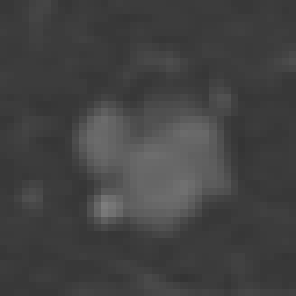
\includegraphics[width=12mm]{figs/ct}};
\node[lbl] at (3.40,-2.05) {Image};

\fill[fm] (4.45,0.85) rectangle (4.61,1.75);
\fill[fm] (4.73,0.98) rectangle (4.89,1.62);
\fill[fm] (5.01,1.08) rectangle (5.17,1.52);
\node[lbl] at (4.81,0.60) {Prior Net};

\latentmap{6.60}{1.30}{0.7}
\node[lbl] at (6.60,0.42) {$p(z\mid x)$};
\latentmap{9.00}{1.30}{0.7}
\node[lbl,anchor=west] at (8.70,0.42) {$q(z\mid x,Y_g)$};

\fill[fm] (8.56,3.00) rectangle (8.72,3.80);
\fill[fm] (8.92,3.08) rectangle (9.08,3.72);
\fill[fm] (9.28,3.15) rectangle (9.44,3.65);
\node[lbl] at (9.00,4.05) {Posterior Net};

% U-Net: encoder down, decoder up, sampled z (green) wedged between the last
% decoder block and the final 1x1 block, exactly as in the paper.
\fill[fm] (5.66,-1.50) rectangle (5.82,-0.30);
\fill[fm] (6.06,-1.70) rectangle (6.22,-0.80);
\fill[fm] (6.46,-1.85) rectangle (6.62,-1.25);
\fill[fm] (6.86,-2.00) rectangle (7.14,-1.60);
\fill[fm] (7.38,-1.85) rectangle (7.54,-1.25);
\fill[fm] (7.78,-1.70) rectangle (7.94,-0.80);
\fill[fm] (8.18,-1.50) rectangle (8.34,-0.30);
\fill[pgreen!35,draw=black!45,line width=0.3pt] (8.34,-1.50) rectangle (8.50,-0.30);
\fill[fm] (8.50,-1.50) rectangle (8.66,-0.30);
\draw[->,blue!55!black,line width=0.4pt] (5.82,-0.45) -- (8.18,-0.45);
\draw[->,blue!55!black,line width=0.4pt] (6.22,-0.90) -- (7.78,-0.90);
\draw[->,blue!55!black,line width=0.4pt] (6.62,-1.35) -- (7.38,-1.35);
\node[lbl] at (7.20,-2.15) {U-Net};

\blobmap{10.90}{-1.20}{0.6}{1.0}{\blobpath}
\node[lbl,align=center] at (10.90,-2.13) {Predicted\\segmentation};

% the four graders; the one drawn at random as Y_g is outlined in green
\node[pic] at (12.90,-0.88) {
\includegraphics[width=6mm]{figs/mask0}};
\node[pic] at (13.52,-0.88) {
\includegraphics[width=6mm]{figs/mask1}};
\node[pic] at (12.90,-1.50) {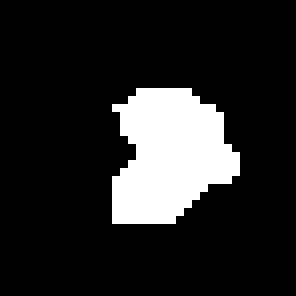
\includegraphics[width=6mm]{figs/mask2}};
\node[pic] at (13.52,-1.50) {
\includegraphics[width=6mm]{figs/mask3}};
\draw[pgreen,line width=1.1pt] (12.60,-1.18) rectangle (13.20,-0.58);
\node[lbl] at (13.21,-2.08) {$Y_1..Y_4$};

% one trunk out of the image, branching to the Prior Net
\draw[flow] (3.40,-0.60) -- (3.40,2.60) -- (8.20,2.60) -- (8.20,3.40) -- (8.56,3.40);
\draw[flow] (3.40,1.30) -- (4.45,1.30);
\draw[flow] (4.00,-1.20) -- (5.66,-1.20);
\draw[flow] (5.17,1.30) -- (5.90,1.30);
\draw[flow] (9.00,3.08) -- (9.00,2.00);
\draw[loss] (7.30,1.30) -- (8.30,1.30);
\node[lbl] at (7.80,1.48) {KL};
\draw[flow] (8.42,0.60) -- (8.42,-0.30);
\node[lbl,anchor=east] at (8.34,0.04) {Sample $z$};
\draw[flow] (8.66,-1.20) -- (10.30,-1.20);
\draw[loss] (11.50,-1.20) -- (12.60,-1.20);
\node[lbl] at (12.05,-0.32) {cross-entropy};
\draw[flow] (13.21,-0.58) -- (13.21,3.40) -- (9.44,3.40);

% ============ OUR EXTENSION ============
% Side by side, NOT a diagonal stack: overlapping tiles hide the shapes behind
% them, and the whole point of showing several is that they visibly differ.
\blobmap{15.42}{0.90}{0.28}{0.70}{\sampleApath}
\blobmap{16.00}{0.90}{0.28}{0.70}{\sampleBpath}
\blobmap{16.58}{0.90}{0.28}{0.70}{\sampleCpath}
\node[olbl] at (16.00,1.50) {$Q^{(1)},\dots,Q^{(K)}$};

\ringmap{18.80}{0.90}
\node[lbl,anchor=west] at (19.50,0.90) {$U$};

\node[pic] at (18.80,-1.20) {
\includegraphics[width=12mm]{figs/dgt}};
\node[lbl,anchor=west] at (19.50,-1.20) {$D^{GT}$};

\draw[pours,thick,rounded corners=2pt,fill=pours!8]
      (14.95,-3.75) rectangle (17.05,-3.05);
\node[lbl] at (16.00,-3.40) {$1{\times}1$ conv $+\ \sigma$};

\ringmap{18.80}{-3.40}
\node[lbl,anchor=west] at (19.50,-3.40) {$\hat D$};

% F(x) taps the decoder BEFORE z is injected, so it keeps the deeper lane and
% never has to cross the branch that re-runs the network with prior samples.
\draw[oflow] (8.26,-1.50) -- (8.26,-3.40) -- (14.95,-3.40);
\node[olbl] at (11.60,-3.66) {$F(x)$, before $z$};
% NOTE: these K passes re-run the network with z drawn from the PRIOR, not the
% posterior z that produced the prediction above. Labelled on the arrow itself,
% because the arrow leaves the decoder and would otherwise imply the same z.
\draw[oflow] (8.58,-1.50) -- (8.58,-2.50) -- (16.00,-2.50) -- (16.00,0.62);
\node[olbl] at (12.00,-2.72) {$K$ passes with $z_k\sim p(z\mid x)$};
\draw[oflow] (13.82,-1.20) -- (18.20,-1.20);
\draw[oflow] (16.86,0.90) -- (18.20,0.90);
\draw[oflow] (17.05,-3.40) -- (18.20,-3.40);

\draw[loss] (18.80,0.30) -- (18.80,-0.60);
\node[lbl,anchor=east] at (18.65,-0.15) {$L_{\text{align}}$};
\draw[loss] (18.80,-2.80) -- (18.80,-1.80);
\node[lbl,anchor=east] at (18.65,-2.30) {$L_D$};

\end{tikzpicture}}
% Kept deliberately short: Section 2 already states the method, so the caption
% only orients the reader and records the two things the drawing encodes that
% the text cannot show. Resist re-expanding it -- figure + caption is already
% about two thirds of a text block.
\caption{\textbf{The disagreement-aware Probabilistic U-Net (training).}
Outside the dashed box, the original model: its posterior sees the image and
\emph{one} randomly drawn grader $Y_g$ (green outline), and its sampled $z$
(green block) enters the decoder before the final $1{\times}1$ convolutions.
Inside, our extension. $D^{GT}$ --- the normalized binary entropy of the four
graders' per-pixel mean --- peaks in a rim where they disagree; we supervise
$\hat D$ against it with $L_D$ (MSE) and $U$ with $L_{\text{align}}$ ($\ell_1$),
the term that places predictive diversity where annotators actually disagree.
Two things the drawing encodes: $F(x)$ is tapped \emph{before} $z$, so $\hat D$
depends on the image alone; and the $K$ passes behind $U$ draw fresh $z_k$ from
the \emph{prior}, not the posterior $z$ that produced the prediction. The CT
crop, the four masks and $D^{GT}$ are real data (\texttt{LIDC-IDRI-0217});
the predicted segmentation, $U$ and $\hat D$ are schematic, and feature-map
blocks are reduced for clarity.}
\label{fig:model}
\end{figure}


It is worth saying how the two views fit together. $\Dgt$ and $U$ are per-pixel
marginals, that is, projections of the distribution over whole masks that the
paper models. We do not replace one with the other. The conditional VAE still
produces the distribution, the KL term still keeps the prior broad and the
decoded samples coherent, and $L_{\text{align}}$ only says where the variance
should sit. $U$ itself is computed from the $K$ decoded samples, so it is a
readout of that distribution rather than a second, independent pixel-wise model.
There is a limit to this. Four masks fix the per-pixel statistics exactly, so
with $G=4$ the map $\Dgt$ can only take the values $\{0,\,0.81,\,1\}$, but they
say much less about which pixels vary together, so a per-pixel constraint is
close to all that four annotations can support.

This gives two testable claims. \textbf{Q1:} where annotators will disagree is
predictable from the image alone, so $\hat D$ should approximate $\Dgt$ and beat
a trivial predictor that only marks lesion boundaries. \textbf{Q2:} adding
$L_{\text{align}}$ should increase the agreement between $U$ and $\Dgt$ compared
with the baseline, without hurting segmentation quality or the energy distance.

We considered two alternatives. Conditioning the prior on disagreement,
$p(z\mid x,\hat D)$, was rejected because $\hat D$ is itself a deterministic
function of $x$, so it adds no new information and would blur the comparison
between arms. Per-rater output heads or annotator confusion
matrices~\cite{zhang2020} were rejected because the LIDC release does not record
which radiologist produced which mask, and the four raters differ from scan to
scan, so a per-rater parameterisation would have nothing stable to learn.

% ===============================================================
\section{Methodology}\label{sec:method}

\paragraph{Model.} We reimplemented the Probabilistic U-Net in PyTorch, since the
official release is an older TensorFlow codebase that no longer runs on Colab.
The model has three parts. The U-Net is a standard encoder--decoder with skip
connections: the encoder halves the spatial resolution four times while doubling
the channel count, starting from 32 channels, and the decoder mirrors it,
concatenating the matching encoder feature map at every step. Alongside it are
two small convolutional encoders that each output the mean and variance of a
six-dimensional Gaussian. The prior encoder sees only the image; the posterior
encoder, used during training, sees the image together with one grader's mask. A
sampled $z$ is broadcast into a six-channel spatial map, concatenated onto the
U-Net's last feature map, and passed through three $1\times1$ convolutions (the
\texttt{fcomb}) that mix the two and produce the class logits. Only this last
block has to be recomputed to draw another sample, which is what makes sampling
cheap. Our disagreement head is a fourth branch: one $1\times1$ convolution and a
sigmoid on that same last feature map, taken before $z$ is concatenated. It lives
in a subclass of the baseline model, so all three arms share one implementation.

\paragraph{Data.} We use the LIDC-IDRI~\cite{lidc} 2D crops from DeepMind's preprocessed
release (CC BY 3.0), published with the Hierarchical Probabilistic
U-Net~\cite{kohl2019}, whose preprocessing follows Appendix H.1 of the original
paper. The splits contain 8843 training, 1993 validation and 1980 test images
from 530, 111 and 103 patients respectively; images are $180\times180$ 8-bit
grayscale with four masks each. We take a random $128\times128$ crop, scale
images to $[0,1]$ and binarise the masks. These counts are up to 0.6\% below the
8882 / 1996 / 1992 reported in the paper, because the authors cleaned the dataset
after publication and the 2018 snapshot was never released. About 65\% of
training crops contain at least one empty mask, which reflects disagreement about
whether a lesion exists at all rather than about where its boundary lies. This
turns out to matter for how the metrics are computed.

\paragraph{Training.} The objective, optimiser and schedule are taken unchanged
from the original paper: the reconstruction cross-entropy summed over pixels,
$\beta=1$ with a six-dimensional latent, Adam with learning rate $10^{-4}$
decayed to $10^{-6}$ in five steps, batch size 32 and weight decay $10^{-5}$. We
did not tune any of these, and every arm uses them identically, which is what
lets the results be read as an ablation rather than as the outcome of a search.

Three choices were ours. We train for 100k steps instead of the paper's 240k,
which was a matter of available compute. Our absolute numbers are therefore not
directly comparable with the published ones, but since all three arms were
trained for the same number of steps, comparing them with each other is still
fair. We set $\lambda_D=0.01$ and $\lambda_A=10^{-5}$ after short 10k-step
trials over a range of values, which showed that larger weights on the auxiliary
terms buy very little and cost a great deal: at $\lambda_A=10^{-3}$ the
uncertainty correlation improved by roughly $0.02$ while Dice fell from $0.30$ to
$0.12$. We kept the smallest weights that still had a measurable effect. Finally,
we clip the gradient norm at 100 and clamp the latent log-variance, both needed
to keep training stable. Augmentation is limited to the random translated crop,
where the paper also uses elastic deformation, rotation, shearing and scaling.
Training draws $K=4$ samples per step and evaluation uses 16 samples per image.

\paragraph{Ablation design.} Three arms vary one component at a time.

\begin{center}\small
\begin{tabular}{llll}
\toprule
Arm & Disagreement head & Alignment loss & Objective \\
\midrule
A -- baseline PU-Net & no  & no  & $L_{\text{PU-Net}}$ \\
B -- $+$ head        & yes & no  & $+\lambda_D L_D$ \\
C -- full model      & yes & yes & $+\lambda_D L_D+\lambda_A L_{\text{align}}$ \\
\bottomrule
\end{tabular}
\end{center}

\paragraph{Tools.} Python, PyTorch, NumPy and Matplotlib. The submitted code runs
in Google Colab as a self-contained notebook that executes the whole pipeline in
a reduced configuration for a quick demonstration; the same code, run at full
length, produced every number reported below.

% ===============================================================
\section{Results and analysis}\label{sec:results}

\paragraph{Metrics.} Dice and IoU, with
$\mathrm{Dice}(A,B)=2|A\cap B|/(|A|+|B|)$, check that the extension does not
damage segmentation quality. We compute them between the model's deterministic
prediction and each of the four masks in turn. They are not our headline claim.
The generalized energy distance compares our 16 samples with the four human
masks. Because both IoU and Dice are $0/0$ when the two masks being compared are
empty, some convention is needed for those pairs. For the energy distance we
follow the paper's Appendix~B, which sets $d\equiv0$, so that agreeing there is
no lesion counts as agreement. The paper does not say what to do for Dice, and
there we made our own choice: we drop empty-versus-empty pairs from the average
rather than scoring them zero. Scoring them zero would penalise every model
equally on the 65\% of crops that contain an empty mask and would hide the
differences we care about. The correlation $\mathrm{corr}(U,\Dgt)$, which asks
whether the model is uncertain in the same places the humans disagree, is our
primary result.

Two further diagnostics are needed. Disagreement in LIDC concentrates on lesion
boundaries, so a map that merely marks a boundary already correlates with $\Dgt$.
We therefore compare $\hat D$ against a trivial control: a 5-pixel band around
the edge of the model's own predicted mask, reaching about two pixels inside and
two outside. The control uses no grader information at all, so unlike a band
drawn around the ground truth it is something a deployed model could actually
compute. We also report the $\mathrm{E}[d(S,S')]$ term of the energy distance on
its own, since it detects samples that have collapsed onto a single mask, and
\emph{nestedness}: the fraction of images for which, after sorting that image's
samples by area, each one is wholly contained in the next. Nestedness catches a
subtler failure, where the model only inflates and shrinks one shape without ever
proposing a different one, so its samples can look varied while really having a
single degree of freedom.

\paragraph{Main results.} Table~\ref{tab:main} reports the held-out test split
(1980 images, 16 samples per image), with every arm read from its 100k-step
checkpoint.

\begin{table}[h]
\centering\footnotesize\setlength{\tabcolsep}{4.5pt}
\begin{tabular}{lcccccccc}
\toprule
Arm & Dice $\uparrow$ & IoU $\uparrow$ & GED $\downarrow$ &
  $\mathrm{corr}(U,\Dgt)\uparrow$ & $\mathrm{corr}(\hat D,\Dgt)\uparrow$ &
  control & $\mathrm{E}[d(S,S')]$ & nested $\downarrow$ \\
\midrule
A -- baseline        & \textbf{0.355} & \textbf{0.280} & 0.394 & 0.483 & --- & 0.417 & 0.686 & 1\% \\
B -- $+$ head        & 0.308 & 0.241 & 0.403 & 0.492 & 0.609 & 0.451 & 0.687 & 3\% \\
C -- full            & 0.340 & 0.267 & \textbf{0.388} & \textbf{0.509} & \textbf{0.627} & 0.425 & 0.692 & 1\% \\
\bottomrule
\end{tabular}
\caption{Test-set results. \emph{control} is the boundary-band predictor for the
same model, so $\mathrm{corr}(\hat D,\Dgt)$ should be read against the value
beside it.}
\label{tab:main}
\end{table}

Q1 holds. The head reaches $\mathrm{corr}(\hat D,\Dgt)=0.627$ against its own
boundary-band control of $0.425$, a margin of $+0.20$, and the same pattern
appears in both arms that carry a head. The head has therefore learned something
about how the annotators behave, not merely retraced the outline of its own
prediction. This is the clearest positive result we obtained.

Q2 is supported, but the effect is small. The correlation
$\mathrm{corr}(U,\Dgt)$ rises from $0.483$ to $0.509$ between arms A and C, and
arm C at the same time reaches the best energy distance of the three ($0.388$)
for a 4\% relative drop in Dice. We think the modest size of the gain is
structural rather than a matter of tuning. $L_{\text{align}}$ can only see the
per-pixel marginal, so two sample distributions that share a marginal look
identical to it: the loss can move variance around, but it cannot change which
masks the model proposes.

Getting even this far required fixing a bug in our own implementation. Our
\texttt{fcomb} originally applied no nonlinearity between its $1\times1$
convolutions, which made the whole block a single affine map. Since $z$ enters as
a spatially constant vector, every sample was then a level set of one fixed
function, and 100\% of test images had strictly nested samples: $z$ could only
grow or shrink one mask, never move part of a boundary and leave the rest. With
the activations applied, nestedness drops to the 1--3\% in Table~\ref{tab:main},
and only then does the alignment loss have anything to act on.

\begin{figure}[!ht]
\centering
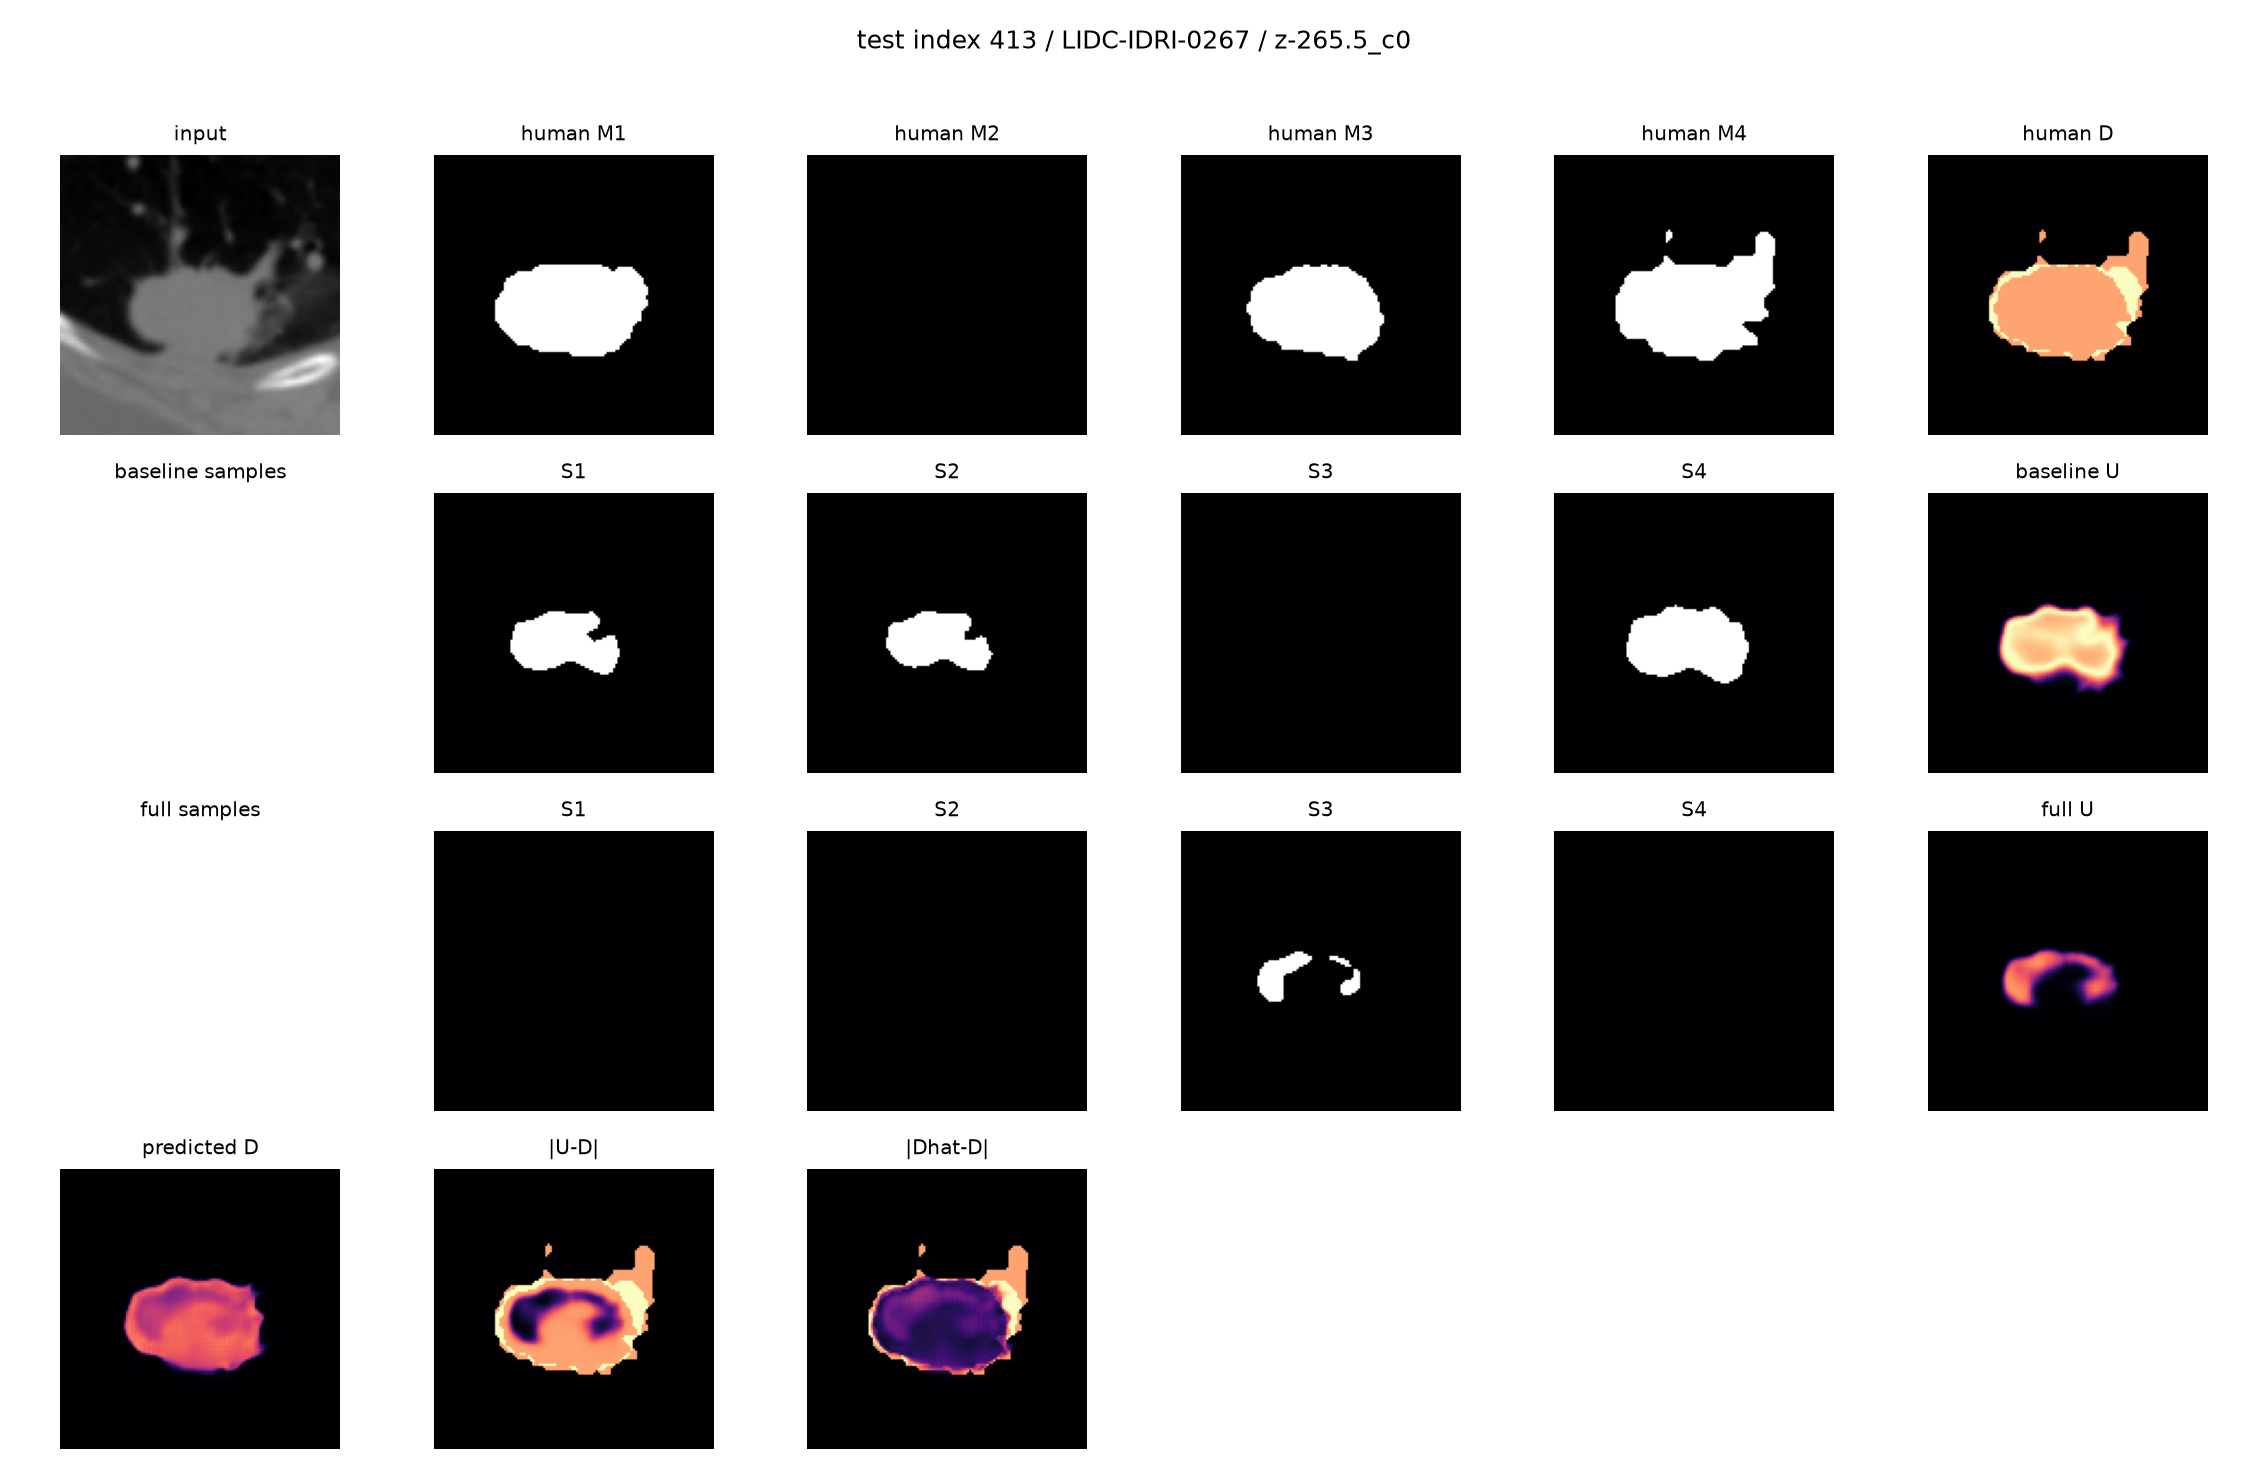
\includegraphics[width=0.86\textwidth]{figs/qualitative}
\vspace{-0.6em}
\caption{A case where the graders disagree about whether a lesion exists at all
(test index 413, LIDC-IDRI-0267). Row 1 shows the CT crop, the four expert masks,
of which M2 is empty, and $\Dgt$, which covers the whole nodule rather than a rim
because the disagreement is about existence rather than boundary placement. Row 2
shows four segmentations sampled from the baseline and the uncertainty map $U$
they produce; row 3 shows the same for our full model. Both reproduce the
ambiguity, in that some of their samples contain the nodule and some are empty.
Row 4 shows the predicted $\hat D$ and the two error maps. $|\hat D-\Dgt|$ is
dark over the lesion while $|U-\Dgt|$ is bright: the head recovers this kind of
disagreement, but $U$ would have to be maximal across the entire nodule to match
$\Dgt$, which pulls directly against the segmentation loss.}
\label{fig:qual}
\end{figure}

\paragraph{Challenges.} The most instructive problem was a posterior collapse in
our first full-length run, which we discarded. We had averaged the reconstruction
cross-entropy over pixels where the original paper~\cite{kohl2018} sums it. At
$128\times128$ that under-weights the reconstruction by a factor of about 16000
against $\beta\,\mathrm{KL}$, so $\beta=1$ behaved like $\beta\approx16000$. The
KL term reached zero by step 31k and the validation energy distance rose from
$0.34$ to $0.61$ while Dice kept improving, which is the signature of a network
that has quietly become deterministic. Summing the cross-entropy fixed it, and it
was a useful reminder that in a VAE the reduction used for the reconstruction
term is not a formatting detail.

Checkpoint selection turned out to be misleading in a similar way. Choosing the
checkpoint with the best validation energy distance picks step 1000 for arm A and
step 3000 for arm B, because a barely-trained model with a wide, uninformative
prior scores well on that metric. We therefore report all arms at the same 100k
steps, which compares the methods rather than how long they happened to train.

Finally, Figure~\ref{fig:qual} points at a limit of the idea itself. Much of the
disagreement in LIDC is about whether a nodule is there at all, so asking $U$ to
match $\Dgt$ asks the model to be maximally uncertain across whole lesions, which
works directly against the reconstruction term. This bounds how far
$L_{\text{align}}$ can usefully be pushed.

% ===============================================================
\section{Conclusion}\label{sec:conc}

We set out to make a Probabilistic U-Net say not just how much its samples should
vary but where. Two findings came out of it. Where radiologists will disagree is
predictable from the image alone: a single $1\times1$ convolution reaches a
correlation of $0.627$ with the true disagreement map, against $0.425$ for a
trivial boundary-band predictor. Aligning the sample diversity with that
disagreement gives a smaller but consistent gain, raising $\mathrm{corr}(U,\Dgt)$
by $0.026$ while reaching the best energy distance of our three arms at a 4\%
Dice cost. The claim we want to make is not that our Dice is higher; the baseline
already produces diverse plausible segmentations. It is that our version puts
that diversity where the experts actually disagree, and makes the disagreement
itself an output one can look at.

The main limitation is that $\Dgt$ and $U$ are per-pixel quantities. Two graders
drawing one mask and two drawing a clearly different one can produce the same
$\Dgt$ as four graders disagreeing pixel by pixel, so neither map distinguishes
two coherent interpretations from unstructured noise. This bounds both what we
can supervise and what we can measure. Beyond that, we trained for 100k of the
paper's 240k iterations and used only the random crop for augmentation, so our
absolute energy distances sit above the published ones; we tested one dataset and
one anatomy; $\Dgt$ is estimated from just four graders; and each arm was run
once, with a single seed, so the smaller differences between arms, including arm
B's lower Dice, cannot be separated from run-to-run variation.

Two directions look worth taking. Restricting $L_{\text{align}}$ to a band around
the predicted boundary would let it shape where edges are drawn without demanding
uncertainty across whole lesions, which we think is the most likely route to a
clearer Q2 result. It would also be informative to compare against the
Hierarchical Probabilistic U-Net, a follow-up by the same authors that models
ambiguity at several spatial scales instead of through one global latent, and
which we would expect to handle existence-versus-boundary disagreement better
than our single six-dimensional $z$.

% ===============================================================
{\footnotesize
\begin{thebibliography}{9}\setlength{\itemsep}{0pt}
\bibitem{kohl2018} S.~A.~A. Kohl et al., \emph{A Probabilistic U-Net for
Segmentation of Ambiguous Images}, NeurIPS 2018. arXiv:1806.05034.
\bibitem{kohl2019} S.~A.~A. Kohl et al., \emph{A Hierarchical Probabilistic U-Net
for Modeling Multi-Scale Ambiguity}, 2019. arXiv:1905.13077. (Source of the
preprocessed LIDC crops.)
\bibitem{lidc} S.~G. Armato~III et al., \emph{The Lung Image Database Consortium
(LIDC) and Image Database Resource Initiative (IDRI)}, Medical Physics, 2011.
\bibitem{ronneberger2015} O.~Ronneberger, P.~Fischer, T.~Brox, \emph{U-Net:
Convolutional Networks for Biomedical Image Segmentation}, MICCAI 2015.
\bibitem{zhang2020} L.~Zhang et al., \emph{Disentangling Human Error from the
Ground Truth in Segmentation of Medical Images}, NeurIPS 2020.
\end{thebibliography}}

\end{document}
